\section{Results}
\label{sec:results}

\begin{figure}[t]
\centering
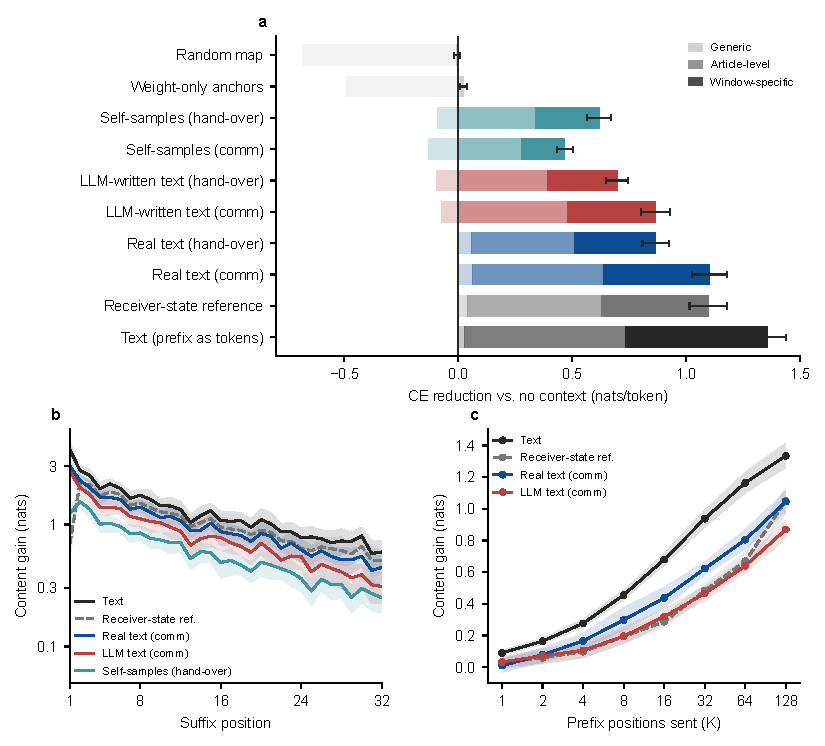
\includegraphics[width=\linewidth]{figs/fig_comm.pdf}
\caption{\textbf{What a latent message is worth to the receiver} (pythia-70m layer 2 $\to$ pythia-160m layer 1; $B$ sees only the 32-token suffix). \textbf{a}, Reduction in $B$'s suffix cross-entropy relative to no context on 493 test windows from 54 WikiText-103 articles (windows inside one article that have a same-article donor), decomposed with donor messages (\S\ref{sec:protocol}): generic (a message from another article), article-level (another window of the same article, minus another article) and window-specific (own window, minus a same-article window). Negative generic parts are drawn left of zero. Error bars: 95\% interval of the content part (article-level + window-specific) from a bootstrap over articles, fitting seeds and donor draws. \textbf{b}, Content gain at each suffix position (log scale) and \textbf{c}, when only the last $K$ prefix positions are sent (for text, $B$ reads the last $K$ prefix tokens); both use all 512 windows and one other-article donor per window, with pointwise 95\% article-bootstrap bands.}
\label{fig:comm}
\end{figure}

\subsection{Choosing where to bridge}
\label{sec:where}
The protocol fixes an injection depth $L_B$, and everything $B$ computes below it on the suffix is computed without the prefix. Injecting $B$'s own prefix states shows what this costs (Appendix~\ref{app:ceiling}): with pythia-160m as $B$, this reference reaches \CEILLONE\% next-token accuracy at $L_B=1$ but only \CEILLSIX\% at $L_B=6$, against \CEILFULL\% with the full prefix and \CEILNONE\% with none. Mid-depth hand-over, the usual stitching configuration, leaves little room for communication. We selected $(L_A, L_B)$ on the WikiText \emph{validation} split with a short real-text fit (Appendix~\ref{app:sweep}): $L_A=2$, $L_B=1$ minimised validation cross-entropy, with $L_A=1$--3 close behind. Mapping $A$'s final hidden state (after its output layer norm) gave the worst validation cross-entropy at both $L_B$ (4.64 and 4.55, against 4.03). \FREESWEEP

\subsection{A valid control needs donors from other documents}
\label{sec:generic}
Swapping messages between examples is the natural control for latent communication \citep[cf.][]{du2025interlat}, but which examples supply the swapped message matters. Our first analysis rolled messages within each batch of 16 windows. Because test windows are sorted by text position, 83\% of those donors came from the same article (427 of 512), and the control attributed 54\% of the real-text bridge's benefit (0.59 of 1.10 nats) to ``generic'' context. With donors drawn from other articles, the generic part of the same bridge is 0.06 nats [0.03, 0.10], or 6\% of its benefit (Figure~\ref{fig:comm}a). For text it is 0.03 nats [$-$0.00, 0.06] of a 1.36-nat benefit. Nearly all of the benefit of a real prefix or a real-text bridge is therefore content, and about half of that content is shared across windows of the same article (article-level 0.71 and window-specific 0.62 nats for text). A same-article donor removes that shared half along with the generic part. The decompositions below use donors from other articles and from the same article (five random draws of each per window, donors restricted to windows inside one article), evaluated on the 493 recipient windows that lie inside one article and have a same-article donor, so that generic, article-level and window-specific parts sum exactly to the total. Intervals come from a bootstrap that resamples articles, fitting seeds and donor draws.

\subsection{Bridges fitted on synthetic text deliver most of the receiver-state reference}
\label{sec:datafree}
Table~\ref{tab:comm} reports the decomposition for every message source. We compare against the \emph{receiver-state reference}, $B$'s own prefix states injected the same way. The reference is not an upper bound (a bridge could supply states that suit the spliced computation better), but it is a natural yardstick: it is what $B$ itself would have sent. We report two ratios: of content gains, which isolates what depends on the particular prefix, and of total gains, which also counts how the receiver fares with an irrelevant message.

\emph{A real-text bridge comes close to the reference.} With the communication objective, its content gain is 1.04 nats against the reference's 1.06, a ratio of 0.99 [0.94, 1.03] (per seed 0.94, 1.01, 1.01); its total gain is 1.00 [0.97, 1.04] of the reference's. A linear map from a 70M model's layer-2 states thus lets a 160M receiver predict the suffix about as well as its own layer-1 states would. Panel~b shows how the profile differs: at the first suffix position the bridged message is far more useful than the reference, while later positions fall slightly below it. One possible reason is that $A$'s layer-2 states have mixed in more of the prefix than $B$'s layer-1 states; we did not test this.

\emph{LLM-written text gets 82\% of the reference's content.} Fitted on 382k characters of encyclopedia-style text written by an LLM with no access to any corpus, the communication-objective bridge reaches a content gain of 0.86 nats: 0.82 [0.79, 0.85] of the reference (per seed 0.80, 0.81, 0.85) and 0.83 of the real-text bridge. Counting total gain, the ratio is lower, 0.72 [0.68, 0.76], because synthetic-text bridges have a \emph{negative} generic part: with a message about a different article, $B$ does worse on average than with no message at all ($-0.07$ nats [$-0.11$, $-0.04$] for LLM-written text, $-0.13$ for self-samples), whereas real-text bridges help slightly even then. Is this harm a general weakness of the receiver, or of the hidden-state interface? Neither: given an unrelated article's prefix \emph{as text}, $B$ does not get worse on average (generic part $+0.03$), and neither does it with an unrelated article's receiver-state reference ($+0.04$) or an unrelated message through the real-text bridge ($+0.06$). Paired per window against the text channel, the irrelevant-message effect differs by $+0.01$ [$-0.00$, 0.03] for the reference, $+0.03$ [0.02, 0.05] for the real-text bridge, but $-0.10$ [$-0.12$, $-0.08$] for the LLM-text bridge and $-0.16$ [$-0.17$, $-0.14$] for the self-sample bridge; averaged over seeds and donors, an irrelevant message worsens CE in 66\% and 81\% of windows for these two, against 48\% for irrelevant text (intervals from an article bootstrap, conditional on the saved fits and donor draws). For this pair and domain, the extra fragility is specific to bridges fitted on synthetic text. It is not universal: in other settings irrelevant messages also hurt through real-text bridges (generic part $-0.07$ with pythia-410m as receiver, $-0.02$ on reviews, $-0.35$ on code) and even as text ($-0.18$ with pythia-410m as receiver, $-0.26$ on code; Appendix~\ref{app:general}). Relative to the real-text bridge, the LLM-text bridge's shortfall of 0.31 nats splits into 0.17 [0.14, 0.21] of content and 0.13 [0.11, 0.16] of generic gain.

\emph{Self-samples and weight algebra fall far short.} Bridges fitted on samples from $A$ and $B$ themselves reach 0.44 [0.42, 0.47] of the reference's content with the communication objective and 0.59 [0.55, 0.62] with the hand-over objective. The best LLM-text bridge exceeds the best self-sample bridge by 0.25 nats [0.21, 0.28] of content; under matched objectives the margins are 0.40 [0.36, 0.44] (communication) and 0.08 [0.04, 0.11] (hand-over). The probe pools differ in more than their source (8.8M characters of real text; 382k characters, 88k tokens, of LLM text; 512 sampled sequences, 82k tokens, of self-samples), so these comparisons are between recipes, not between text sources at equal budget; \S\ref{sec:scale} compares real and LLM-written text at equal size. The weight-only least-squares map reaches a content gain of 0.02 nats [0.01, 0.04], 2\% of the reference, together with a generic loss of 0.49 nats. The random map shows no detectable content gain ($-0.01$ [$-0.02$, 0.01]).

\begin{table}[t]
\centering\small
\caption{Communication setting, pythia-70m L2 $\to$ pythia-160m L1, on 493 test windows (54 articles) that lie inside one article and have a same-article donor. Suffix CE in nats/token; gains relative to $B$ with no context (CE 4.930). Generic + content = total gain; the split of content into article-level and window-specific parts is shown in Figure~\ref{fig:comm}a. Content and net ratios divide a bridge's content and total gains by those of the receiver-state reference. 95\% intervals from a bootstrap over articles, fitting seeds and donor draws (4000 draws); fitted bridges average three seeds, all conditions average five donor draws of each kind.}
\label{tab:comm}
\resizebox{\linewidth}{!}{\footnotesize\setlength{\tabcolsep}{3pt}\begin{tabular}{lccccc}
\toprule
Message source (objective) & Total & Generic & Content & Content ratio & Net ratio \\
\midrule
Random map & $-$0.690 & $-$0.684 & $-$0.006 [$-$0.019, 0.007] & $-$0.01 [$-$0.02, 0.01] & $-$0.63 [$-$0.68, $-$0.59] \\
Weight-only anchors & $-$0.469 & $-$0.491 & 0.022 [0.005, 0.039] & 0.02 [0.00, 0.04] & $-$0.43 [$-$0.46, $-$0.40] \\
\midrule
Self-samples (hand-over) & 0.525 & $-$0.093 & 0.618 [0.566, 0.672] & 0.59 [0.55, 0.62] & 0.48 [0.45, 0.52] \\
Self-samples (comm) & 0.338 & $-$0.129 & 0.467 [0.434, 0.504] & 0.44 [0.42, 0.47] & 0.31 [0.29, 0.33] \\
LLM-written text (hand-over) & 0.601 & $-$0.096 & 0.697 [0.649, 0.746] & 0.66 [0.64, 0.68] & 0.55 [0.52, 0.57] \\
LLM-written text (comm) & 0.792 & $-$0.073 & 0.865 [0.803, 0.930] & 0.82 [0.79, 0.85] & 0.72 [0.68, 0.76] \\
Real text (hand-over) & 0.866 & 0.059 & 0.807 [0.750, 0.866] & 0.76 [0.74, 0.80] & 0.79 [0.76, 0.82] \\
Real text (comm) & 1.102 & 0.062 & 1.040 [0.963, 1.116] & 0.99 [0.94, 1.03] & 1.00 [0.97, 1.04] \\
\midrule
Receiver-state reference & 1.097 & 0.042 & 1.055 [0.974, 1.138] & 1 & 1 \\
Text (prefix as tokens) & 1.357 & 0.028 & 1.329 [1.247, 1.410] & 1.26 [1.23, 1.29] & 1.24 [1.21, 1.27] \\
\bottomrule
\end{tabular}
}
\end{table}

\subsection{Per transmitted position, the latent message is worth less than text}
\label{sec:bandwidth}
Hidden states are often assumed to carry more than the tokens they sit on. For this receiver and these bridges, that is not what we measure. At full length, the receiver-state reference delivers 79\% of the content gain that text delivers (1.06 vs 1.33 nats; Table~\ref{tab:comm}); one difference between the two is that with the message, $B$'s first layer processes the suffix without the prefix. When only the last $K$ prefix positions are sent (Figure~\ref{fig:comm}c), $K$ tokens of text are worth more than $K$ bridged positions at every tested $K\in\{1,2,4,\dots,128\}$: the difference between text and the real-text bridge ranges from 0.08 nats [0.04, 0.12] at $K=1$ to 0.36 [0.30, 0.43] at $K=64$, and all eight Bonferroni-adjusted intervals exclude zero (smallest lower bound 0.02; intervals resample articles and are conditional on the saved bridges and one other-article donor draw). This is an operational result for this receiver, not a statement about information density. Short messages also change other things: the bridges were fitted only on 128-position messages, a truncated message places a mid-document state at sequence position 0, and absolute cross-entropy with a short latent message is \emph{worse} than with no context (Appendix~\ref{app:bandwidth}). Bridges trained for short messages, or receivers that inject at several layers or into key--value caches \citep{fu2026c2c}, may behave differently.

Equal numbers of positions are not equal communication costs. Payload: a 128-position message costs 262\,kB in float32 if $A$'s 512-dimensional states are sent and the bridge is applied at the receiver (131\,kB in float16), or 393\,kB if the bridged 768-dimensional states are sent; 128 token ids packed as 16-bit integers cost 256 bytes, so the latent message is about three orders of magnitude larger. Computation: in an idealised split implementation the receiver still runs 11 of its 12 layers on every message position, roughly the same as reading the prefix as text (a dense-layer estimate of $2\times85$M non-embedding parameters $\times128$ positions $\approx 22$ GFLOP either way), and the sender adds two of its layers; our implementation runs both models in full and overwrites states, so it does not realise even that. We did not measure latency. This design therefore shows no communication-efficiency advantage; the case for latent channels rests on settings where the sender would otherwise have to \emph{generate} text token by token, the motivation of \citet{fu2026c2c} and \citet{zou2025latentmas}, which we do not test.


\subsection{How far the findings generalise}
\label{sec:scale}

Table~\ref{tab:general} repeats the measurement across model pairs, model families and test domains. The content contrast can grow because matched messages help more or because irrelevant messages hurt more, so for each bridge we report both its content ratio and its \emph{net} ratio: the total reduction in cross-entropy relative to no context, divided by the reference's. Appendix~\ref{app:general} lists the populations and protocol differences.

\begin{table}[t]
\centering\small
\caption{Generalisation. For each bridge, content gain (other-document donor minus matched message) and net gain (no context minus matched message), each relative to the receiver-state reference of the same receiver on the same windows; reference content in nats. 95\% intervals over documents, fitting seeds and donor draws. All bridges use the communication objective; layer pairs were selected on validation text for each model pair. The code and review rows evaluate the main pair's bridges, fitted on WikiText-like text, without refitting. Too few review windows have a same-document donor to split content into article-level and window-specific parts (Appendix~\ref{app:general}).}
\label{tab:general}
{\footnotesize\setlength{\tabcolsep}{4pt}\begin{tabular}{llccc}
\toprule
Setting & Probe text & Ref.\ content & Content ratio & Net ratio \\
\midrule
Pythia 70M$\to$160M (main) & Real text & 1.06 & 0.99 [0.94, 1.03] & 1.00 [0.97, 1.04] \\
 & LLM text &  & 0.82 [0.79, 0.85] & 0.72 [0.68, 0.76] \\
 & Self-samples &  & 0.44 [0.42, 0.47] & 0.31 [0.29, 0.33] \\
\addlinespace
Pythia 410M$\to$160M & Real text & 1.06 & 1.02 [0.98, 1.06] & 0.99 [0.96, 1.03] \\
 & LLM text &  & 0.89 [0.86, 0.92] & 0.70 [0.67, 0.73] \\
 & Self-samples &  & 0.55 [0.45, 0.65] & 0.31 [0.22, 0.40] \\
\addlinespace
Pythia 160M$\to$410M & Real text & 1.51 & 0.85 [0.79, 0.91] & 0.87 [0.82, 0.92] \\
 & LLM text &  & 0.77 [0.75, 0.80] & 0.69 [0.67, 0.72] \\
 & Self-samples &  & 0.27 [0.24, 0.34] & 0.14 [0.09, 0.17] \\
\addlinespace
GPT-2$\to$Pythia 160M & Real text & 1.05 & 1.02 [0.98, 1.05] & 1.00 [0.97, 1.03] \\
 & LLM text &  & 0.87 [0.78, 0.93] & 0.70 [0.61, 0.76] \\
 & Self-samples &  & 0.70 [0.66, 0.74] & 0.54 [0.51, 0.58] \\
\addlinespace
GPT-2$\to$Qwen2.5 0.5B & Real text & 1.58 & 0.50 [0.25, 0.76] & 0.62 [0.44, 0.80] \\
 & LLM text &  & 0.57 [0.46, 0.67] & 0.43 [0.34, 0.52] \\
\addlinespace
OPT 125M$\to$GPT-2 & Real text & 1.40 & 0.28 [0.26, 0.30] & 0.65 [0.60, 0.71] \\
 & LLM text &  & 0.28 [0.25, 0.31] & 0.27 [0.22, 0.32] \\
\addlinespace
Code (70M$\to$160M) & Real text & 1.26 & 0.31 [0.26, 0.34] & 0.03 [$-$0.03, 0.10] \\
 & LLM text &  & 0.30 [0.27, 0.32] & $-$0.10 [$-$0.16, $-$0.03] \\
 & Self-samples &  & 0.30 [0.28, 0.31] & 0.21 [0.19, 0.24] \\
\addlinespace
Reviews (70M$\to$160M) & Real text & 0.43 & 0.81 [0.76, 0.87] & 0.71 [0.65, 0.76] \\
 & LLM text &  & 0.73 [0.70, 0.76] & 0.63 [0.60, 0.67] \\
 & Self-samples &  & 0.46 [0.43, 0.50] & 0.46 [0.42, 0.50] \\
\bottomrule
\end{tabular}
}
\end{table}

\paragraph{The receiver's own states are matched only in some pairs.} In-domain, the real-text bridge's net ratio is close to 1 when pythia-70m, pythia-410m or GPT-2 sends to pythia-160m (1.00, 0.99 and 1.00). It is lower, 0.87 [0.82, 0.92], when pythia-160m sends to pythia-410m, a receiver whose own states are far more useful (1.51 nats of content, 93\% of what text gives it). The shortfall could come from the sender, the bridge's capacity or optimisation, or the restricted layer search, since the selected sender layer was the deepest candidate; we cannot tell these apart. The main pair shows that a less capable sender is not by itself an obstacle.

\paragraph{No net improvement was detected with a stronger sender.} We replaced pythia-70m by pythia-410m as sender to the same receiver, on identical windows and donors. The LLM-text bridge's content ratio rises from 0.82 to 0.89, but the net gain does not change detectably for any probe source, and its point estimates are slightly lower. For real text, LLM text and self-samples, the net gain changes by $-0.01$ [$-0.06$, 0.04], $-0.03$ [$-0.07$, 0.01] and $-0.00$ [$-0.09$, 0.11] nats, and the content gain by $+0.03$ [$-0.03$, 0.11], $+0.07$ [0.04, 0.11] and $+0.11$ [$-0.01$, 0.22]. The bootstrap pairs fitting seeds across senders, which share probe and minibatch seeds, and uses identical donor draws. Only the LLM-text bridge's content change is detectably positive, and in these fits its larger contrast reflects worse predictions with irrelevant messages rather than better ones with relevant messages. Read alone, the content contrast would suggest an improvement that the net gain does not show.

\paragraph{Other model families.} \XFAMILYRESULTS

\paragraph{Other domains.} The main pair's bridges were fitted for encyclopedia-like text. On long IMDB reviews (at least 322 tokens, 30\% of the test split), the domain's own reference is weaker, with 0.43 nats of content, and the bridges keep most of its content and net gain. Their content and net ratios are 0.81 and 0.71 for real text, 0.73 and 0.63 for LLM text, and 0.46 and 0.46 for self-samples.

On Python source code, all three retain about 30\% of the reference's content, but their net effects diverge. The self-sample bridge still helps (net ratio 0.21 [0.19, 0.24]), the real-text bridge's effect is unresolved (0.03 [$-0.03$, 0.10]), and the LLM-text bridge leaves the receiver worse off than no message ($-0.10$ [$-0.16$, $-0.03$]). On code, even an unrelated file's prefix given as text hurts the receiver (generic part $-0.26$). Relative performance falls sharply on this corpus, and which bridge is useful there is not predicted by which is best in-domain.

\paragraph{Text source and amount.} \TEXTSOURCES

\paragraph{Bridge capacity.} \CAPACITY

\subsection{Hand-over stitching answers a different question}
\label{sec:diag}
In the classical hand-over setting, $B$ reads the tokens, but the bridged $A$ state replaces every layer-$L_B$ state. Bridged systems score below $A$ alone on accuracy, both here and on two small testbeds (Appendix~\ref{app:small}). Table~\ref{tab:diag} varies optimisation length, bridge capacity and layer pairing for 70M$\to$160M. It uses a real-text probe, one seed and 512 test windows. We interpret this diagnostic descriptively because it uses a single seed and checkpoints chosen post hoc.

\begin{table}[h]
\centering\small
\caption{Hand-over setting, pythia-70m $\to$ pythia-160m: next-token accuracy (\%) / cross-entropy (nats) over all 128 positions; one seed. $A$ alone: 25.65 / 4.626; $B$ alone: 30.60 / 4.074. Bridges start from the weight-only map and are trained with Adam at a constant learning rate of $10^{-3}$; the 1500- and 3000-step entries are checkpoints of the same run.}
\label{tab:diag}
\begin{tabular}{lccc}
\toprule
& 600 steps & 1500 steps & 3000 steps \\
\midrule
L3$\to$L6, linear & 21.67 / 4.785 & 23.61 / 4.615 & 22.69 / 4.706 \\
L3$\to$L6, linear + MLP (2048) & 22.38 / 4.710 & 23.82 / 4.582 & 24.64 / 4.535 \\
\midrule
\multicolumn{4}{l}{Depth-matched pairs, linear, 600 steps:} \\
\quad L1$\to$L2 / L2$\to$L4 & \multicolumn{3}{c}{22.44 / 4.786 \qquad 19.71 / 4.998} \\
\quad L4$\to$L8 / L5$\to$L10 & \multicolumn{3}{c}{23.00 / 4.712 \qquad 23.40 / 4.702} \\
\quad L6 (final, after the output layer norm)$\to$L12 & \multicolumn{3}{c}{13.70 / 6.178} \\
\bottomrule
\end{tabular}
\end{table}

No configuration reaches $B$ alone, and none exceeds $A$'s accuracy. The longest-trained non-linear bridge nevertheless has \emph{lower} cross-entropy than $A$ alone, at 4.535 against 4.626. Whether a stitched system ``performs worse than the sender'' therefore depends on the metric and on training, and this observation does not establish a bound: in principle, a downstream decoder can use a representation better than the sender's own upper layers do.

Training length and capacity matter too. At 3000 steps, the non-linear bridge closes 75\% of the accuracy gap between the 600-step linear bridge and $A$ alone. With a constant learning rate, the linear map's accuracy is not monotone in training length: 23.61 at 1500 steps and 22.69 at 3000. Comparisons between stitches based on single checkpoints therefore require caution.

$A$'s final hidden state, taken after its output layer norm, is a poor source both here and in the communication setting (\S\ref{sec:where}). We did not test the pre-normalisation final residual state, so these results say nothing about the information present before $A$'s last normalisation.

In the communication setting, $B$ keeps its own suffix computation and receives only what it lacks. We ask whether the message improves $B$ beyond the benefit of any message. Comparing the stitched system with either model answers a different question.


